% Rapport Sandillon (M1, 2024). Compiler dans outils/rapports/restauration :
%   Rscript figures.R && ../compiler.sh restauration
\documentclass[11pt,a4paper]{article}
\usepackage{../rapport-portfolio}
\definecolor{themehex}{HTML}{9A6A22}\colorlet{theme}{themehex}
\addbibresource{references.bib}

\titrerapport{Restauration des habitats de la carrière de Sandillon (Loiret)}
\titrecourt{Restauration de la carrière de Sandillon}
\soustitre{Flore et carabes comme bioindicateurs de deux sites réaménagés comparés à un témoin}
\auteurs{Claire Bellin et Jérémy Genty}
\cadre{Master 1 BICG · UE Écologie de la restauration · Université d'Orléans}
\annee{Rapport d'étude · 2023-2024}
\motcle{Écologie de la restauration}
\visuel{\photogarde{figures/photo_fosse.jpg}}
\creditvisuel{Fosse réaménagée en 2016 : les talus sont taillés pour la nidification de l'hirondelle de rivage.}

\begin{document}
\pagedegarde

\enbref{Les deux sites exploités puis remis en état (2006 et 2016) portent la même végétation de friche que le témoin jamais exploité, avec des flores proches (Jaccard 0,38 à 0,44). Chez les carabes, le témoin reste le plus diversifié : à effort égal (102 individus), on y attend 22 espèces, contre 15 à 18 sur les sites restaurés. La remise en état restaure donc la végétation plus vite que la faune du sol, et les talus aménagés en 2016 accueillent l'hirondelle de rivage.}

\section{Introduction}
L'effondrement de la biodiversité à l'échelle mondiale fait aujourd'hui consensus, et les milieux anthropisés deviennent eux aussi des lieux de conservation. L'exploitation minière compte parmi les principales perturbations des milieux naturels \parencite{pitz2018} ; la question est alors de savoir quelle approche de restauration adopter après exploitation.

La carrière de Sandillon (Loiret), gérée par le groupe CEMEX, extrait du sable depuis les années 1960-1970. Elle forme une mosaïque de secteurs exploités, en cours d'exploitation ou jamais exploités. Nous y avons comparé deux sites remis en état à des dates différentes à un site témoin jamais exploité, afin d'évaluer l'effet de la restauration. Parmi les bioindicateurs suivis (flore, carabes, amphibiens, reptiles, oiseaux), ce rapport porte sur la flore et les carabes.

\section{Matériel et méthodes}
\subsection{Site d'étude}
La carrière produit des granulats pour le béton. L'exploitation suit trois étapes : la terre de surface est décapée sur 20 à 30~cm et mise de côté, le sable est extrait, puis la fosse est remblayée avec des matériaux tout-venant et recouverte de la terre d'origine. Trois sites ont été comparés (figure~\ref{fig:carte}) :
\begin{itemize}
\item une friche dont l'exploitation s'est achevée en 2006, sans aménagement particulier ;
\item une friche achevée en 2016, où des merlons favorables à la nidification de l'hirondelle de rivage ont été aménagés au bord de deux étangs ;
\item une zone témoin jamais exploitée.
\end{itemize}

\begin{figure}[ht]
\centering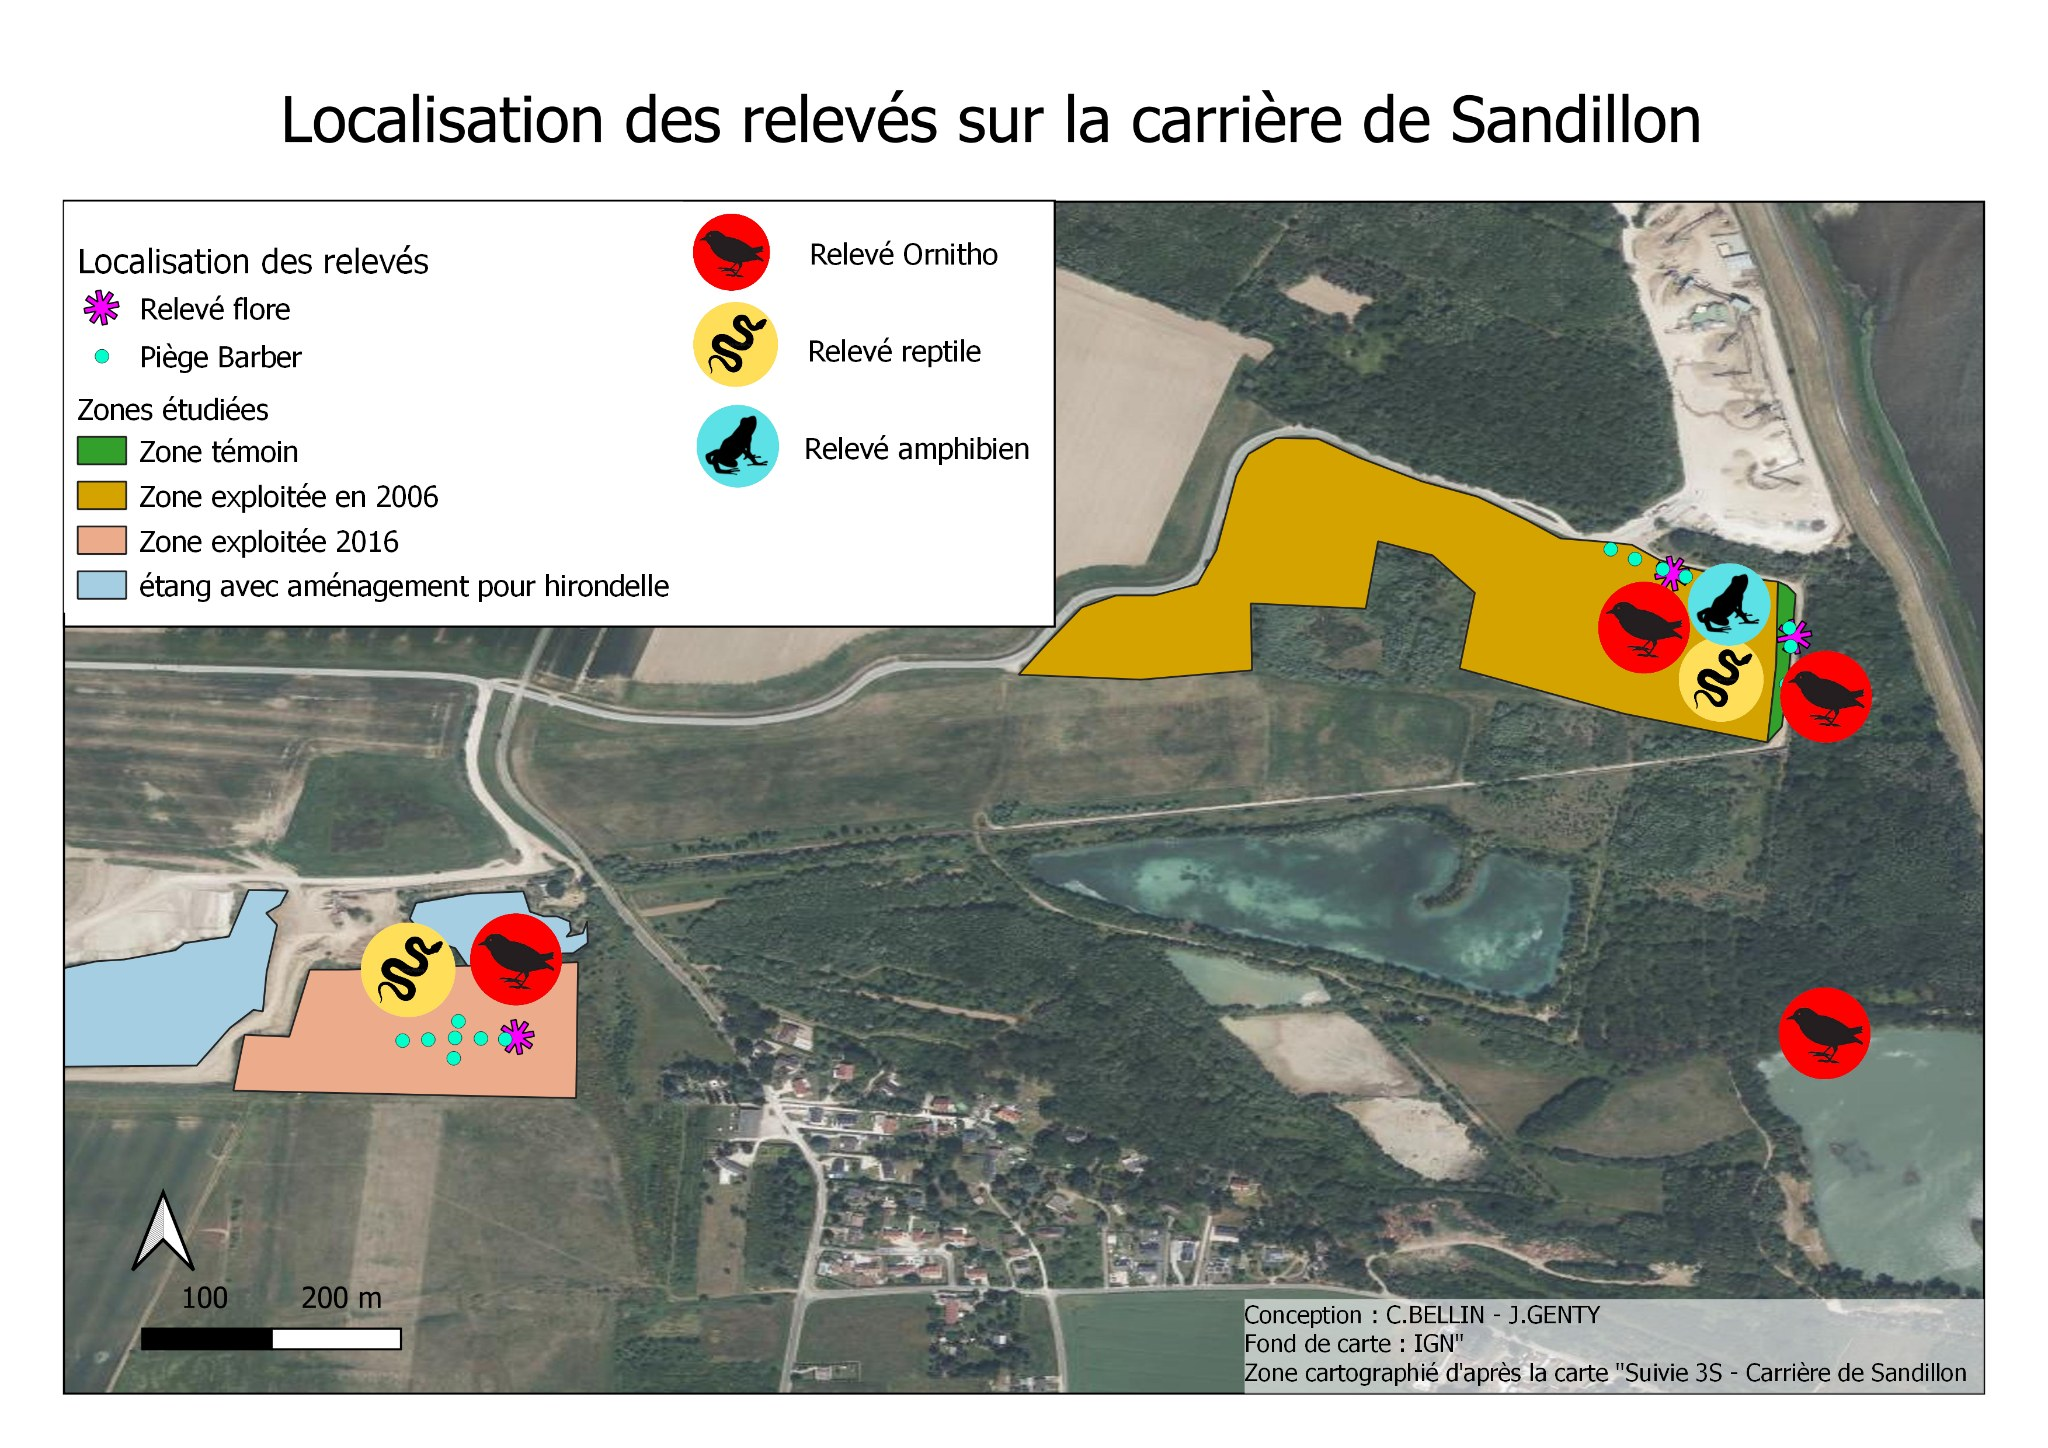
\includegraphics[width=0.88\linewidth]{figures/carte_releves.jpg}
\caption{Localisation des relevés sur la carrière de Sandillon : zones témoin, exploitée jusqu'en 2006 et jusqu'en 2016, et points de relevés par groupe.}
\label{fig:carte}
\end{figure}

\subsection{Protocoles}
Les relevés suivent le protocole ROSELIERE \parencite{parisot2015}, qui fixe les dates et les méthodes. Les oiseaux ont été inventoriés par indices ponctuels d'abondance (IPA) : 20~minutes d'écoute et d'observation à la jumelle et à la longue-vue. Pour les reptiles, des plaques ont été posées et deux mares inventoriées. Les relevés ont eu lieu le 16 février et le 24 avril 2024 (synthèse des oiseaux en annexe).

\subsubsection{Flore}
Sur chaque site, des cercles de 10~m² ont été inventoriés à deux reprises ; les plantes ont été identifiées au genre ou à l'espèce, avec un coefficient d'abondance-dominance \parencite{braunblanquet1932}. Nous avons ensuite :
\begin{itemize}
\item calculé l'indice de Jaccard entre sites, $J = C/(A+B+C)$, où $A$ et $B$ sont les nombres de taxons propres à chacun des deux relevés et $C$ le nombre de taxons communs \parencite{jaccard1901} ;
\item établi les spectres biologiques de Raunkiær \parencite{raunkiaer1904}, réduits ici à la part des vivaces et des annuelles, en présence et en recouvrement ;
\item calculé les valeurs indicatrices moyennes d'Ellenberg \parencite{ellenberg1992} pour l'humidité (F), le pH (R) et la trophie (N), et tracé les écogrammes correspondants ;
\item rattaché chaque relevé à un syntaxon jusqu'à l'association avec le guide des végétations du Centre-Val de Loire \parencite{pujol2023} ;
\item recherché les espèces déterminantes de ZNIEFF, structurantes, protégées et exotiques envahissantes ; les espèces structurantes ont un intérêt fonctionnel ou patrimonial qui oriente la gestion \parencite{chaurand2011}.
\end{itemize}

\subsubsection{Carabes}
Les carabes, très diversifiés et sensibles à l'état du sol, sont de bons bioindicateurs \parencite{chapelin}. Ils sont capturés par des pièges Barber : gobelets enterrés au ras du sol, remplis d'eau et d'un tensioactif inodore, disposés en étoiles de cinq pièges et relevés après deux semaines (figure~\ref{fig:barber}). Les pièges posés en 2024 n'étaient pas encore triés : les analyses portent sur la campagne 2017, avec neuf étoiles sur le site 2006 et cinq sur le site 2016 et sur le témoin.

\begin{figure}[ht]
\centering
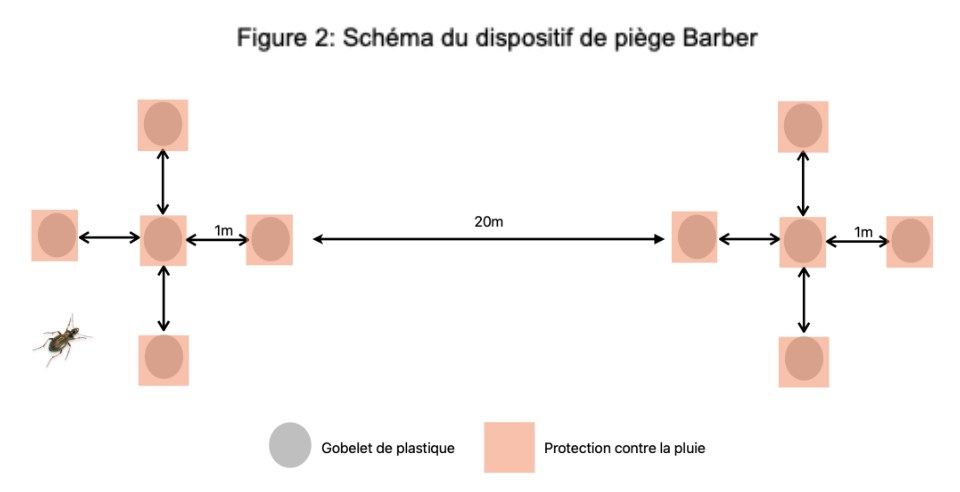
\includegraphics[height=42mm]{figures/schema_barber.jpg}\hfill
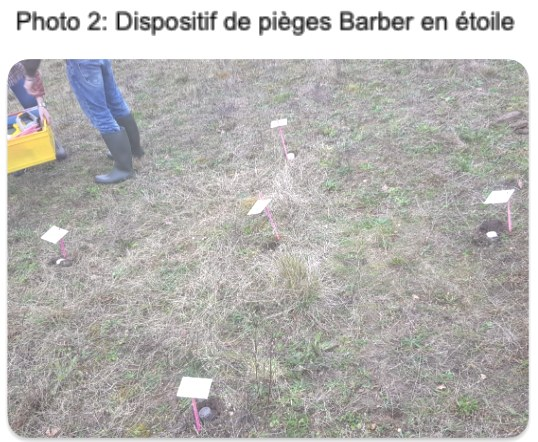
\includegraphics[height=42mm]{figures/photo_barber.jpg}
\caption{Pièges Barber disposés en étoile : schéma du dispositif (à gauche) et pose sur le terrain (à droite).}
\label{fig:barber}
\end{figure}

Les analyses, réalisées avec le package R \emph{vegan}, portent sur l'abondance et la richesse : diagramme rang-abondance, courbe d'accumulation pour juger de l'effort d'échantillonnage, raréfaction pour comparer la richesse à effectif égal. La diversité est résumée par l'indice de Shannon $H$ (nul si une seule espèce, maximal et égal à $\ln S$ si les $S$ espèces sont également abondantes), l'indice de Simpson sous la forme $1-D$ (probabilité que deux individus tirés au hasard appartiennent à deux espèces différentes) et l'équitabilité de Pielou $H/\ln S$ (de 0 à 1).

\section{Résultats : flore}
\subsection{Richesse et similarité}
Le témoin compte 45 taxons, la friche 2006 en compte 52 et la friche 2016, 30. Les indices de Jaccard entre sites vont de 0,38 à 0,44 (moyenne 0,40, tableau~\ref{tab:jaccard}), au-dessus du seuil de 0,2 retenu pour conclure à une flore homogène \parencite{sepant}.

\begin{table}[ht]
\centering\small
\caption{Indice de Jaccard entre sites. $A$ et $B$ : taxons propres au premier et au second site ; $C$ : taxons communs.}
\label{tab:jaccard}
\begin{tabular}{@{}lrrrr@{}}
\toprule\entete
Sites comparés & $A$ & $B$ & $C$ & Jaccard\\
\midrule
Friche 2006 / témoin & 22 & 6 & 17 & 0,38\\
Friche 2016 / témoin & 15 & 7 & 17 & 0,44\\
Friche 2006 / friche 2016 & 20 & 11 & 19 & 0,38\\
\midrule
Moyenne & & & & 0,40\\
\bottomrule
\end{tabular}
\end{table}

\noterevision{Note de révision (2026) : dans la version de 2024, les indices des deux dernières lignes étaient intervertis (0,37 et 0,44) ; ils sont recalculés ici à partir de $A$, $B$ et $C$.}

\subsection{Spectres biologiques}
Les vivaces dominent sur les trois sites, en présence (61 à 68~\% des espèces) comme en recouvrement (figure~\ref{fig:spectres}). La friche 2016 se distingue en recouvrement : les vivaces y couvrent 82~\% de la surface, contre 64 à 66~\% ailleurs.

\begin{figure}[ht]
\centering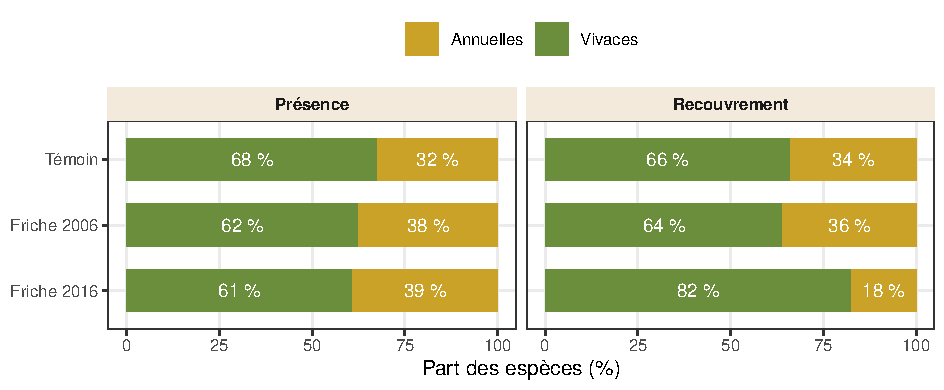
\includegraphics[width=0.9\linewidth]{figures/fig_spectres.pdf}
\caption{Spectres biologiques simplifiés : part des vivaces et des annuelles, en présence et en recouvrement.}
\label{fig:spectres}
\end{figure}

\noterevision{Note de révision (2026) : dans la version de 2024, deux graphiques portaient le titre « Friche témoin, présence » ; le second (60,9~\% de vivaces) est attribué ici à la friche 2016, seule combinaison manquante.}

\subsection{Valences écologiques et écogrammes}
Les valeurs d'Ellenberg moyennes sont très proches entre sites (tableau~\ref{tab:ellenberg}, figure~\ref{fig:eco}). La friche 2006 est un peu plus sèche (F = 4, milieu mésoxérophile) que la friche 2016 et le témoin (F = 5, mésohydriques). Les deux friches exploitées sont neutroclines (R = 6), le témoin un peu plus acide (R = 5). Les trois sites sont mésotrophes (N = 5).

\begin{table}[ht]
\centering\small
\caption{Valeurs indicatrices moyennes d'Ellenberg par site. L : lumière ; T : température ; K : continentalité ; F : humidité ; R : pH ; N : trophie ; S : salinité.}
\label{tab:ellenberg}
\begin{tabular}{@{}lccccccc@{}}
\toprule\entete
Site & L & T & K & F & R & N & S\\
\midrule
Témoin & 7 & 5 & 5 & 5 & 5 & 5 & 1\\
Friche 2006 & 7 & 5 & 5 & 4 & 6 & 5 & 0\\
Friche 2016 & 7 & 5 & 5 & 5 & 6 & 5 & 0\\
\bottomrule
\end{tabular}
\end{table}

\begin{figure}[ht]
\centering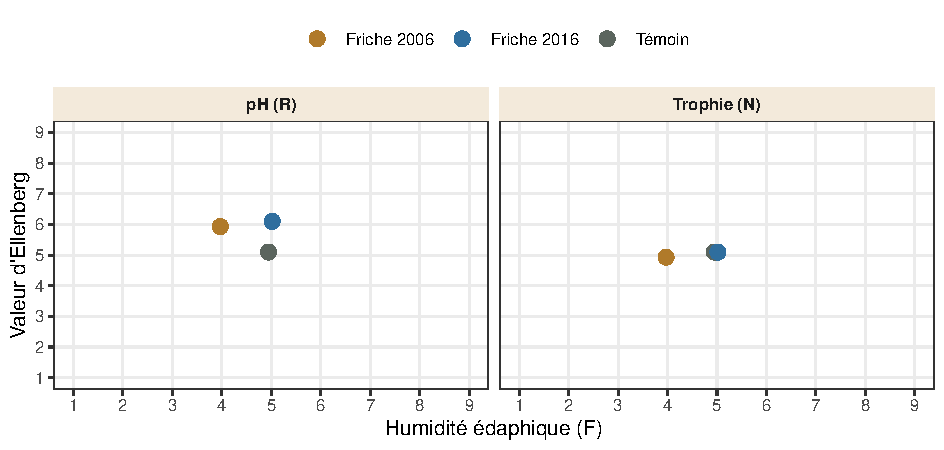
\includegraphics[width=0.9\linewidth]{figures/fig_ecogrammes.pdf}
\caption{Écogrammes : humidité édaphique croisée avec le pH (à gauche) et avec la trophie (à droite).}
\label{fig:eco}
\end{figure}

\subsection{Syntaxon et espèces remarquables}
Les trois sites relèvent du même syntaxon \parencite{pujol2023} : classe des \emph{Artemisietea vulgaris}, ordre des \emph{Onopordetalia acanthii}, alliance du \emph{Dauco carotae-Melilotion albi}, association du \emph{Melilotetum albo-officinalis}. Ce sont des friches de hautes herbes mésothermophiles, en milieu semi-ouvert, sur substrat plus ou moins grossier souvent rapporté.

Deux espèces déterminantes de ZNIEFF ont été relevées : \emph{Cirsium tuberosum} dans la friche 2016 et \emph{Scandix pecten-veneris} dans le témoin. Aucune espèce structurante, protégée ou exotique envahissante n'a été observée.

\section{Résultats : carabes}
\subsection{Abondance et richesse}
La friche 2016 compte le plus d'individus et d'espèces (354 individus, 27 espèces), devant le témoin (102 individus, 22 espèces) et la friche 2006 (176 individus, 18 espèces). Sur les trois sites, quelques espèces dominent et beaucoup sont rares (figure~\ref{fig:rang}).

\begin{figure}[ht]
\centering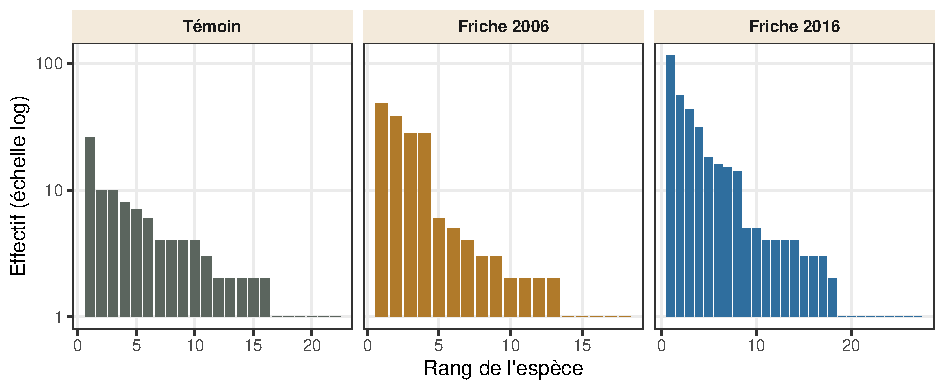
\includegraphics[width=0.95\linewidth]{figures/fig_rang.pdf}
\caption{Diagrammes rang-abondance des carabes (campagne 2017, toutes stations cumulées).}
\label{fig:rang}
\end{figure}

\subsection{Effort d'échantillonnage et raréfaction}
Aucune courbe d'accumulation n'atteint de plateau (figure~\ref{fig:acc}) : l'échantillonnage ne capture pas toute la richesse des sites. La friche 2016 n'est la plus riche qu'en apparence, parce qu'elle a fourni le plus d'individus. À effort égal, ramené aux 102 individus du témoin, la raréfaction donne 22 espèces attendues au témoin, 17,6 sur la friche 2016 et 15,0 sur la friche 2006 (figure~\ref{fig:rar}).

\begin{figure}[ht]
\centering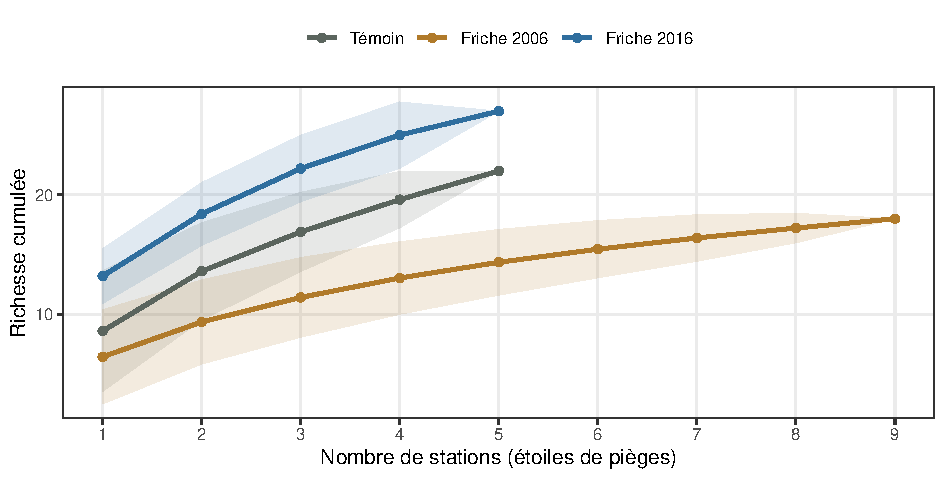
\includegraphics[width=0.78\linewidth]{figures/fig_accumulation.pdf}
\caption{Courbes d'accumulation des espèces selon le nombre de stations (méthode exacte, enveloppe à ±1,96 écart-type).}
\label{fig:acc}
\end{figure}

\begin{figure}[ht]
\centering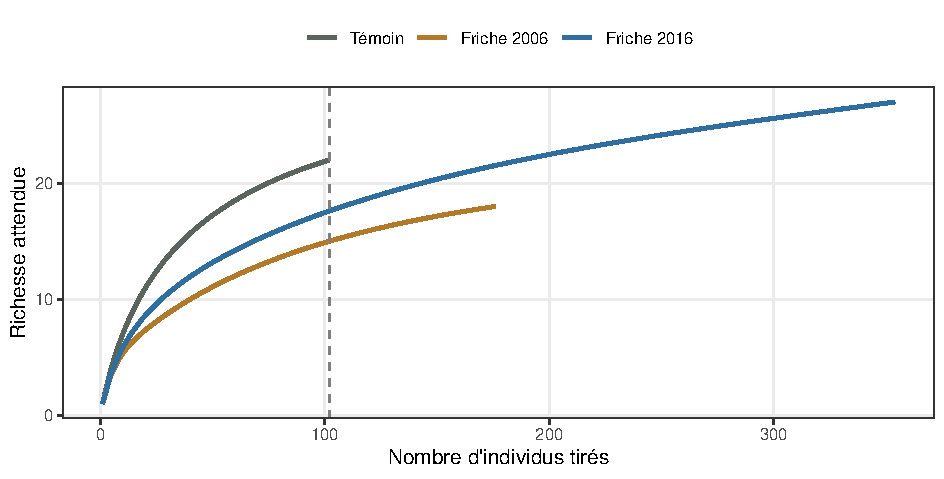
\includegraphics[width=0.78\linewidth]{figures/fig_rarefaction.pdf}
\caption{Courbes de raréfaction par site. Tirets : effectif du témoin (102 individus), qui sert de base de comparaison.}
\label{fig:rar}
\end{figure}

\subsection{Indices de diversité}
Le tableau~\ref{tab:div} donne les indices de deux façons : en moyenne sur les stations, comme dans la version de 2024, et sur les captures cumulées de chaque site. Les deux lectures concordent : la friche 2006 est la moins diversifiée, le témoin le plus équitable. Les valeurs de Simpson proches de 0,8 indiquent qu'aucune espèce n'écrase les autres.

\begin{table}[ht]
\centering\small
\caption{Indices de diversité des carabes : moyenne des stations et valeur sur les captures cumulées du site.}
\label{tab:div}
\begin{tabular}{@{}lcccccc@{}}
\toprule\entete
 & \multicolumn{3}{c}{Moyenne des stations} & \multicolumn{3}{c}{Captures cumulées}\\
\cmidrule(lr){2-4}\cmidrule(l){5-7}\entete
Site & Shannon & Simpson & Pielou & Shannon & Simpson & Pielou\\
\midrule
Témoin & 1,88 & 0,81 & 0,89 & 2,62 & 0,89 & 0,85\\
Friche 2006 & 1,49 & 0,70 & 0,82 & 2,06 & 0,82 & 0,71\\
Friche 2016 & 1,97 & 0,79 & 0,76 & 2,30 & 0,84 & 0,70\\
\bottomrule
\end{tabular}
\end{table}

\noterevision{Note de révision (2026) : la version de 2024 comparait l'indice de Shannon des stations à $\ln S = 3{,}73$, calculé sur les 42 espèces de la carrière, ce qui n'est pas un repère valable pour une station. L'indice de Simpson y était aussi décrit comme la probabilité que deux individus soient de la même espèce, alors que la valeur calculée est son complément. Les analyses ont été refaites à partir des données brutes, avec en plus la raréfaction à effectif égal.}

\section{Discussion}
\subsection{Synthèse des indicateurs}
Le tableau~\ref{tab:synthese} résume la position de chaque site pour les indicateurs étudiés.

\begin{table}[ht]
\centering\small
\caption{Synthèse des indicateurs par site : + valeur élevée, = valeur semblable aux autres sites, - valeur faible.}
\label{tab:synthese}
\begin{tabular}{@{}llccc@{}}
\toprule\entete
Groupe & Indicateur & Témoin & Friche 2006 & Friche 2016\\
\midrule
Flore & Richesse spécifique & + & + & -\\
 & Similarité (Jaccard) & = & = & =\\
 & Spectre biologique (présence) & = & = & =\\
 & Spectre biologique (recouvrement) & = & = & +\\
 & Valences écologiques et syntaxon & = & = & =\\
 & Espèces déterminantes ZNIEFF & + & - & +\\
\midrule
Carabes & Richesse à effort égal & + & - & =\\
 & Diagramme rang-abondance & = & = & =\\
 & Accumulation (plateau atteint) & - & - & -\\
 & Indice de Shannon & + & - & =\\
 & Simpson et Pielou & + & = & =\\
\bottomrule
\end{tabular}
\end{table}

\subsection{Une végétation restaurée, une faune du sol en retard}
Pour la flore, les sites restaurés ne se distinguent presque pas du témoin : similarité élevée, mêmes valences écologiques, même syntaxon. Le témoin est lui-même une friche, ce qui relativise la comparaison : la remise en état ramène la végétation vers celle des friches voisines, pas vers un milieu naturel ancien. La dominance des vivaces signale des milieux en voie de stabilisation \parencite{vincent}, et la présence de deux espèces déterminantes de ZNIEFF montre que le cortège peut gagner en intérêt patrimonial.

Les carabes répondent plus lentement. À effort égal, le témoin reste le plus riche et le plus équitable ; la friche 2006, pourtant la plus ancienne, est la moins diversifiée, peut-être parce qu'elle n'a fait l'objet d'aucun aménagement. Ces écarts restent à confirmer : aucune courbe d'accumulation n'atteint de plateau, et la flore ne repose que sur deux relevés par site. L'aménagement de 2016 a en revanche atteint son but : l'hirondelle de rivage, espèce protégée, a été observée sur la fosse réaménagée (voir l'annexe).

\subsection{Perspectives de gestion}
La restauration peut être active ou passive \parencite{pitz2018}. Ces sols remaniés risquent d'être colonisés par des espèces exotiques envahissantes, qui bloqueraient la succession écologique : un suivi minimal reste nécessaire. L'activité de la carrière peut aussi créer des milieux rares localement : fronts de taille laissés à nu pour les espèces pionnières, sables remis à l'air libre pour des pelouses sableuses, talus pour l'hirondelle de rivage. Il faudrait enfin multiplier les relevés de flore et de carabes, et trier les pièges de 2024, pour suivre l'évolution des sites dans le temps.

\pagebiblio

\clearpage
\section*{Annexe : relevés ornithologiques de 2024}\label{annexe}
\addcontentsline{toc}{section}{Annexe}
Indices ponctuels d'abondance de 20~minutes (observateurs : A. Sallé et M1 BICG). Effectifs observés ou entendus.

\begin{table}[H]
\centering\small
\begin{tabularx}{\linewidth}{@{}llX@{}}
\toprule\entete
Date & Milieu & Espèces (effectif)\\
\midrule
16 février & Friche 2006 & Pic vert (1), Mésange bleue (1), Mésange charbonnière (2), Pinson des arbres (2, en vol), Corneille noire (4), Geai des chênes (1), Pouillot véloce (1), Accenteur mouchet (1)\\
16 février & Étang & Foulque macroule (4), Canard colvert (2), Grèbe huppé (1), Grand Cormoran (2)\\
16 février & Fosse réaménagée 2016 & Canard colvert (2), Fuligule morillon (2), Foulque macroule (2), Vanneau huppé (bande de plus de 10)\\
16 février & Friche 2016 & Alouette des champs (1), Faucon crécerelle (1)\\
24 avril & Fosse réaménagée 2016 & Fuligule morillon (2), \textbf{Hirondelle de rivage (3)}, Vanneau huppé (2)\\
24 avril & Friche 2016 & Alouette des champs (1), Fauvette grisette (1), Bruant jaune (1), Faisan de Colchide (1), Hirondelle de fenêtre (1), Pic vert (1), Corneille noire (1), Pie bavarde (1), Martinet noir (1, en vol), Pigeon ramier (1)\\
\bottomrule
\end{tabularx}
\end{table}
\end{document}
